
\section{Introduction}
One of the most important aspects of machine learning is classification. Typical algorithms and models
that are used for classification include logistic regression, naive bayes, decision trees and so on. In the 90s, 
Vladimir Vapnik and his colleagues developed a new algorithm called \emph{Support Vector Machine (SVM)}.
The name of this algorithm comes from the fact that the algorithm is based on the concept of \emph{support vectors},
which are the data points that are closest to the threshold. This algorithm is dedicated to the classification
of both linearly separable and non-linearly separable data points. In this paper,
we will focus on the main usages of SVM, including the generalization of linear decision boundaries for classification.
We will also discuss the role of kernel in SVM, as well as the implementation, evaluation methods, application and many aspects of SVM.


First, it would be helpful to take a look at an example of a simple data classification problem in a two-dimensional space.
Assume that there are two sets of data points that are separately distributed into two clusters. The classification then
becomes obvious: The threshold that separates both groups simply lies in the middle of the most outward data points
from both groups. This classification method is called the \emph{maximum margin classifier}, since the margin that separates both groups is maximized.

\begin{figure}[h]%
    \begin{center}%
        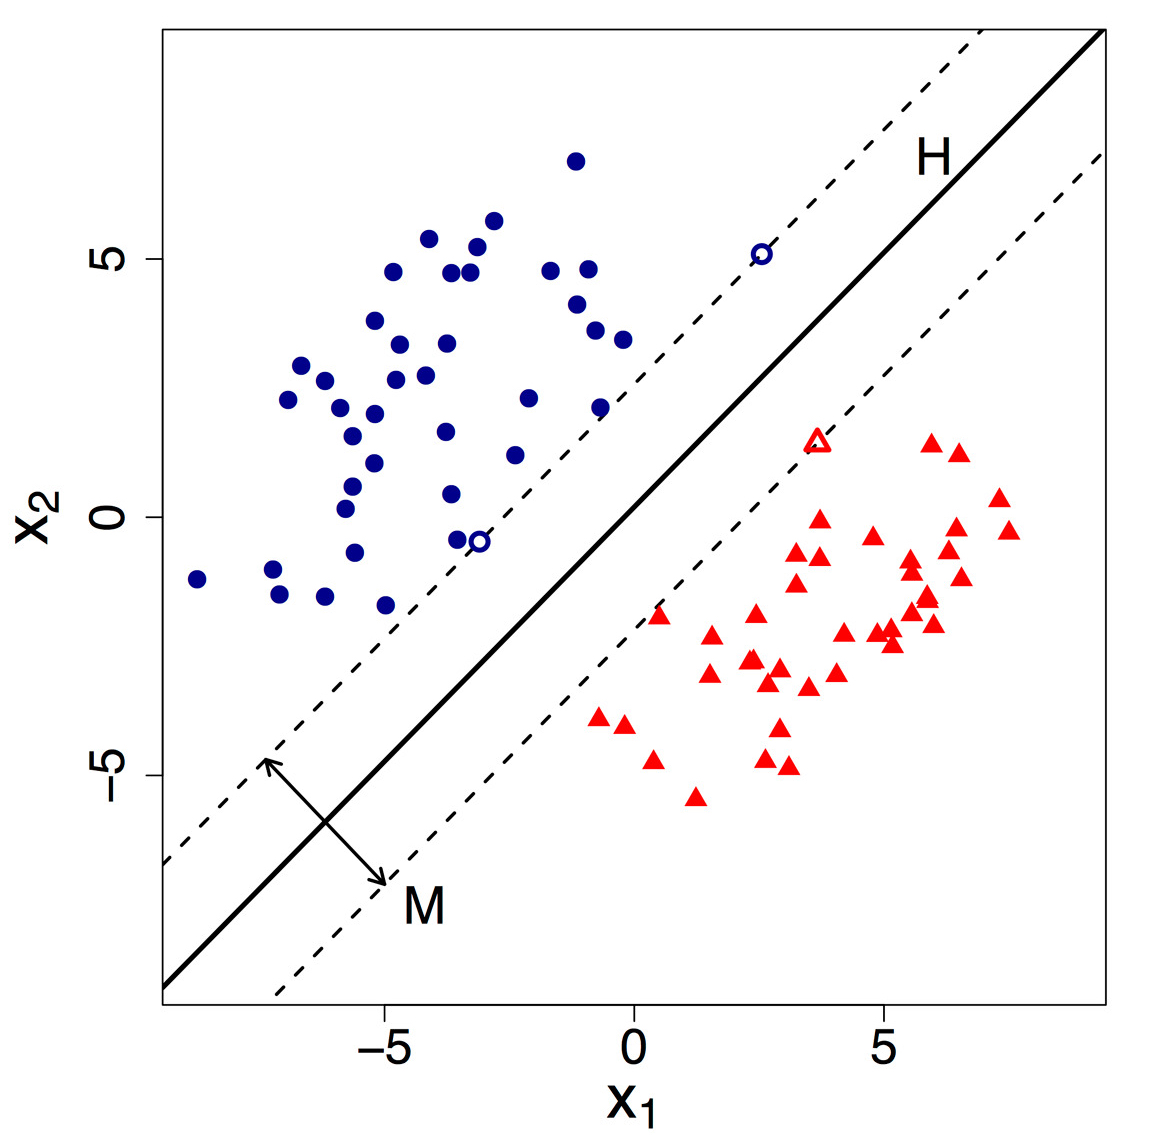
\includegraphics[scale=0.12]{Maximum_Margin_Classifier.jpg}%
        \caption{Maximum Margin Classifier \cite{imgintro}}\label{fig:}%
    \end{center}%
\end{figure}
Nevertheless, the maximum margin classifier is not always applicable, since the data points are not always ideally separable. If an outlier happens to appear in the dataset, it would push the threshold to one side, since the data point
is much closer to the other group. This would result in a severe misclassification, since the data that are close to one
group now belongs to the other group because of the shift of the threshold. A solution to this problem is to allow some
misclassification, so that the threshold is less sensitive to outliers and the classifier performs better
when there is new data. This margin that allows some misclassifications is called the \emph{soft margin} and
the classifier that is used to separate the data points is thus called \emph{soft margin classifier}.
\begin{figure}[h]%
    \begin{center}%
        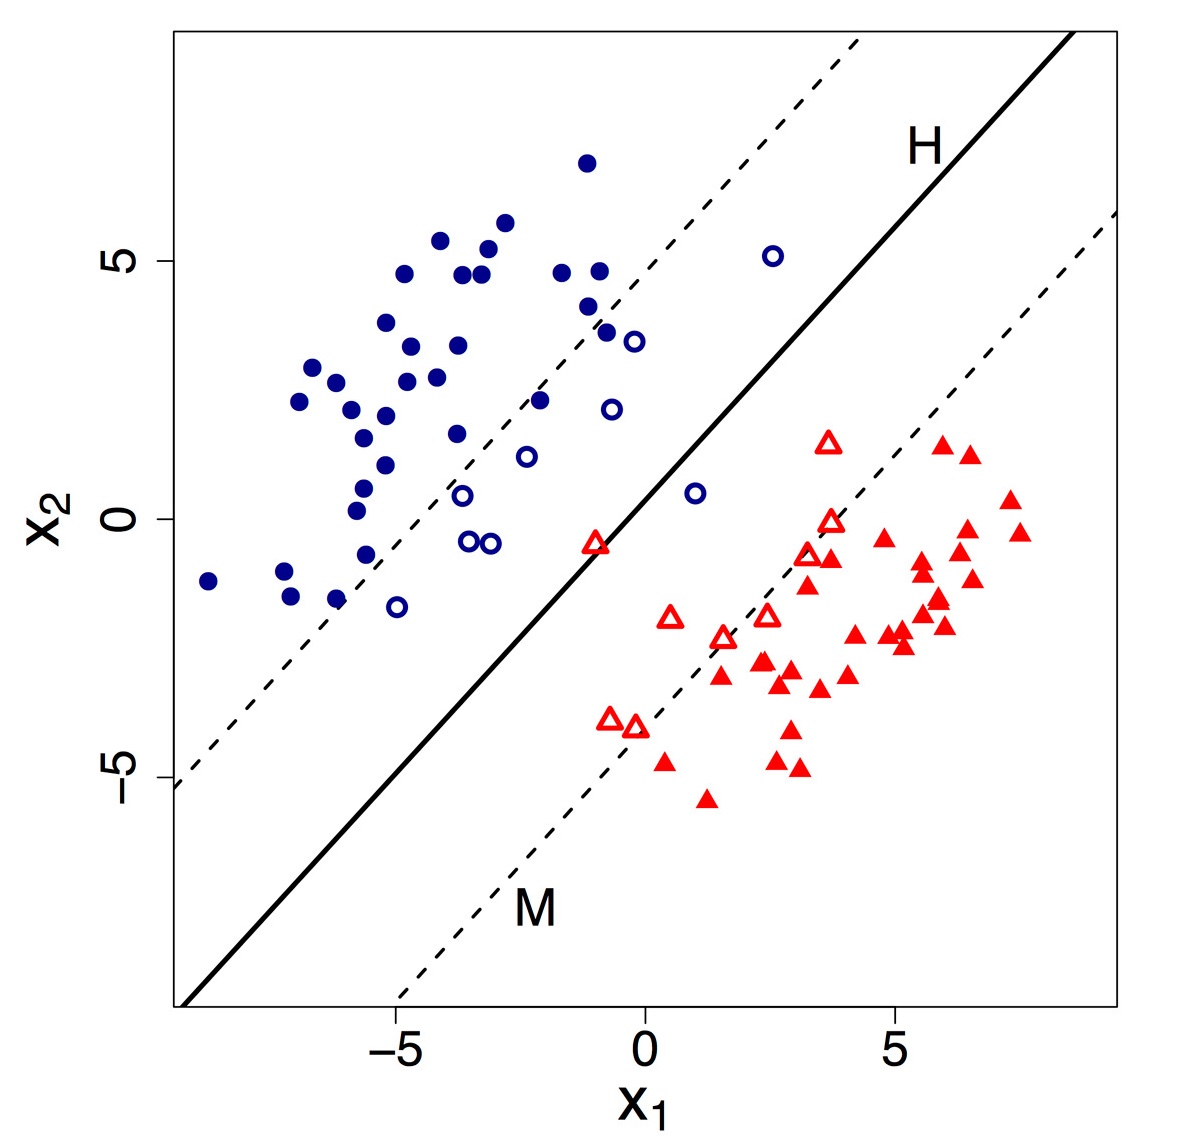
\includegraphics[scale=0.12]{Soft_Margin_Classifier.jpg}%
        \caption{Soft Margin Classifier \cite{imgintro}}\label{fig:}%
    \end{center}%
\end{figure}

For the real life application, nevertheless, the most dataset that we work with is 
most likely not going to be one-dimensional. Due to the multidimensional property of the dataset,
we use vectors and matrices to represent the data. In this case, the idea of hyperplane is introduced. 

A \emph{hyperplane} is a flat affine subspace that is one dimension lower than the ambient space.\cite{R9}
It is used to separate the data in multidimensional space. The soft margin classifier is able to deal with this case as well.
It finds the hyperplane that separates the data in a way that the margin is maximized. We will discuss the exact algorithm and the
mathematics in the next section.

However, the soft margin classifier is still not suitable for data that is not linearly separable, even though 
the soft margin classifiers allow misclassifications and is less sensitive to outliers. Usually, we use a \emph{kernel} to deal 
with this case, which is a function that maps the data into a higher dimensional space, so that the data becomes linearly
separable. The SVM implements the idea of kernel without transforming the data into a higher dimensional space. This concept is 
called \emph{the kernel trick} and is a crucial part of SVM. This trick allows SVM to cast nonlinear variants to dot products,
enabling easier computation and better performance. \cite{Kernel2}
\begin{figure}[h]%
    \begin{center}%
        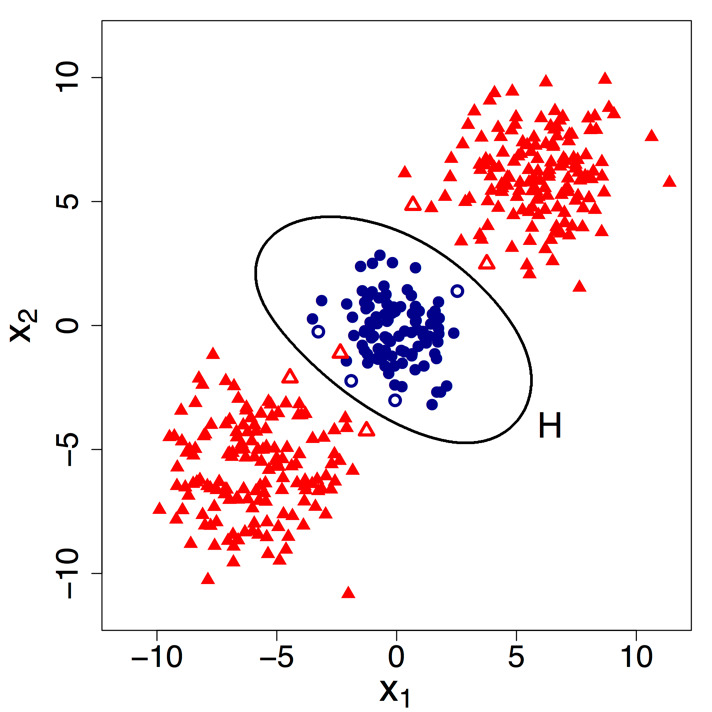
\includegraphics[scale=0.55]{Kernel.jpeg}%
        \caption{Kernel Trick \cite{imgintro}}\label{fig:}%
    \end{center}%
\end{figure}
